\documentclass[conference]{IEEEtran}

\usepackage{cite}
\usepackage{amsmath}
\usepackage{booktabs}
\usepackage{array}
\usepackage{xcolor}
\usepackage{tikz}
\usetikzlibrary{arrows.meta,positioning,fit,backgrounds,calc}
\usepackage{algorithm}
\usepackage[noend]{algpseudocode}
\usepackage[hidelinks]{hyperref}
\usepackage{url}

\newcommand{\cn}[1]{\texttt{#1}}   % condition / code names

\begin{document}

\title{Reducing and Structuring Alive2 Counterexamples for Language-Model-Assisted Repair of LLVM Miscompilations}

\author{%
\IEEEauthorblockN{Abhyuday Vaish}
\IEEEauthorblockA{Vellore Institute of Technology Chennai\\
\texttt{abhyuday.vaish2024@vitstudent.ac.in}}
\and
\IEEEauthorblockN{Bhuvan Nayak}
\IEEEauthorblockA{Vellore Institute of Technology Chennai\\
\texttt{bhuvan.bharatnayak2024@vitstudent.ac.in}}
\and
\IEEEauthorblockN{Siddharth Sameer Nevgi}
\IEEEauthorblockA{Vellore Institute of Technology Chennai\\
\texttt{siddharth.sameer2024@vitstudent.ac.in}}
\and
\IEEEauthorblockN{Tanish Desai}
\IEEEauthorblockA{Vellore Institute of Technology Chennai\\
\texttt{tanish.somashekhar2024@vitstudent.ac.in}}
}

\maketitle

\begin{abstract}
Alive2 can show that an LLVM optimization is not a refinement of its input and print a concrete counterexample. The repair loop of \emph{llvm-apr-benchmark} returns this output to the model as printed, although it contains the whole reproducer, per-value traces for both sides, and verifier boilerplate. We ask whether reducing that counterexample and presenting it in a fixed, structured layout change how often a language model repairs the responsible LLVM C++ code. To study this, we describe a counterexample-processing layer inserted into the repair loop of \emph{llvm-apr-benchmark}. The layer has two independent factors: \emph{reduction} (none, line-level delta debugging, \texttt{llvm-reduce}, or a reducer that edits the source and target IR in tandem using dependency closure and seeds taken from the counterexample, with every edit gated by an Alive2 oracle) and \emph{presentation} (the verifier's text or a deterministic structured rendering). Adding a no-counterexample baseline yields nine conditions. The planned evaluation uses 24 stratified single-function miscompilations, three trials per bug and condition, at most four repair iterations, and exact one-sided McNemar tests over four prespecified comparisons. This paper specifies the method, the implementation, and the evaluation protocol. The experimental sweep has not yet been run, and no repair outcomes are reported.
\end{abstract}

\begin{IEEEkeywords}
compiler testing, translation validation, Alive2, counterexample reduction, program repair, large language models, LLVM
\end{IEEEkeywords}

%=====================================================================
\section{Introduction}
%=====================================================================

When an LLVM middle-end pass miscompiles a function, Alive2 can often demonstrate the error. Given the IR before and after the pass, it searches for an input on which the target does not refine the source, and it reports that input together with the values computed by both sides~\cite{lopes2021alive2}. The repair loop of \emph{llvm-apr-benchmark} returns this report to the model after a failed patch~\cite{zheng2025aprbench}. The report is verbose relative to the information it conveys. It repeats the reproducer pair (the reproducer alone is 6 to 164 lines in the sample used here) and lists every value computed along the failing execution, most of which are unrelated to the violated refinement.

Two lines of work suggest that the form of failure feedback matters. For the repair of ordinary programs, shortening a large failure-inducing test input before it enters the prompt has been reported to help~\cite{yang2026reducefix}, as has selecting the smallest failing counterexample from a pool~\cite{he2026pgs}. For compilers, recent work studies benchmarks and agent harnesses and reports low resolution rates on LLVM bugs~\cite{zheng2026harness,tian2026llvmbench}. Neither line isolates the question that arises when the feedback is a \emph{verifier witness for an IR transformation} and the artifact to repair is the \emph{C++ implementation of the pass}. Does a witness that has been reduced with knowledge of IR structure, and laid out in labelled sections, help the model more than the witness as printed? We treat this as an open empirical question and make no claim about its answer in this paper.

The study varies only the text returned to the model after a failed Alive2 check. Reduction and presentation are separate factors, so that their effects and any interaction can be distinguished. The inherited repair loop, the benchmark, and Alive2 are not contributions of this work. We contribute the following, described in Sections~\ref{sec:method} and~\ref{sec:impl}:
\begin{itemize}
\item a reducer for Alive2 counterexamples that edits source and target in tandem, builds dependency-closed candidates, seeds its search from the verifier's report, and accepts an edit only if an oracle confirms the violation;
\item two baseline reducers that differ from it in what they know about the witness, namely line-level delta debugging and a wrapper around \texttt{llvm-reduce}, so that prompt length and IR validity can be separated from counterexample awareness;
\item a deterministic structured renderer that derives its sections from the IR and the verifier output without a second model; and
\item a nine-condition protocol with a prespecified paired analysis whose resolution limits are stated in advance.
\end{itemize}

The research questions (Section~\ref{sec:problem}) concern whether each factor changes the proportion of bugs repaired, how many repair iterations are needed, and what the reducers cost. All outcome sections of this manuscript are intentionally empty.

%=====================================================================
\section{Background and Related Work}
%=====================================================================

\subsection{Refinement, translation validation, and counterexamples}

LLVM IR is a typed, SSA-based representation whose semantics distinguish immediate undefined behavior (UB) from special values such as \texttt{poison} and \texttt{undef}~\cite{lopes2021alive2,llvmlangref}. Because optimizers exploit UB, correctness is defined as refinement rather than equivalence: the target may be more defined than the source or have fewer behaviors, but never less defined~\cite{lopes2021alive2}. Flags such as \texttt{nsw}, \texttt{nuw}, and \texttt{inbounds} impose additional semantic constraints and can produce poison when their required conditions are violated~\cite{llvmlangref}. Attaching a flag that the source does not justify can therefore break refinement; Alive2's authors report such a case involving \texttt{nsw}~\cite{lopes2021alive2}.

Alive2 checks refinement between pairs of functions with an SMT solver. It unrolls loops to a user-chosen bound, so it can miss violations that require more iterations. It is designed to avoid false alarms, including by over-approximating unsupported features and declining to report a violation that depends on such an approximation~\cite{lopes2021alive2}. It performs the check as a sequence of simpler queries (UB, return domain, poison, undef, value equality, and memory), which supports detailed error messages. Its authors report 47 bugs found by running it over LLVM's unit tests, 28 of which had been fixed at the time of publication~\cite{lopes2021alive2}. Two properties matter for this work. First, a counterexample is a witness under Alive2's bounded semantics, so a reduction that preserves it preserves only that. Second, the printed report is a by-product of the solver query rather than a document written for a reader.

\subsection{Three artifacts that get reduced, and one that gets repaired}

Delta debugging shrinks a failing input by testing subsets and keeping those that still fail. Its \texttt{ddmin} variant stops at a 1-minimal input, from which no single element can be removed, and its authors note that knowledge of the input's structure makes it more effective~\cite{zeller2002dd}. Compiler testing requires reducers that respect validity. Yang et al.\ observed that existing delta-debugging variants for C programs introduced undefined behavior, which produced small programs that no longer demonstrated the bug, and they relied on checkers and manual work to avoid this~\cite{yang2011csmith}. \texttt{llvm-reduce} addresses the same need for IR. It runs delta passes at several granularities against a user-supplied interestingness script and keeps only candidates for which the script exits with status zero~\cite{llvmreducedoc}.

The literature uses ``reduction'' for three distinct artifacts; we distinguish them explicitly.
\begin{enumerate}
\item \emph{Reducing a failing program or input} so that a developer or tool can see the bug. Examples are \texttt{ddmin}, \texttt{llvm-reduce}, and the reducers that users of Csmith depend on~\cite{zeller2002dd,yang2011csmith,llvmreducedoc}. The preserved property is that the program still crashes or miscompiles.
\item \emph{Reducing a failing test input before it enters a repair prompt}. ReduceFix has a model generate a \texttt{ddmin}-based reducer for each task and accepts a reduction only if the buggy and reference programs still disagree on it. It reports a mean size reduction of 89.1\% over successful reductions, on failing inputs whose median size exceeds 1~MB, and pass@10 gains of up to 53.8\% relative to a prompt containing the original test. It also finds that shortening the input contributes more than adding output differences~\cite{yang2026reducefix}. The program under repair is a competitive-programming solution, and the reduced artifact is data that it consumes.
\item \emph{Reducing a verifier witness}, the artifact studied in this paper. The witness is a pair of IR functions plus a report, and the preserved property is a specific refinement violation reported by Alive2. PGS is the nearest relative in the repair literature, but it works differently: it selects the failing counterexample with the fewest input tokens from a pool instead of editing a single counterexample. It reports that minimum-size selection outperformed median and maximum selection, with token count the most effective of three size proxies~\cite{he2026pgs}. Its tasks come from code-generation benchmarks and SWE-bench, not from compiler passes.
\end{enumerate}
What is \emph{repaired} differs again: in this study it is the LLVM C++ that produced the incorrect transformation, not the IR witness.

\subsection{Language-model repair and the form of feedback}

Conversational APR alternates patch generation with validation, incorporating earlier patches and validation feedback into subsequent turns rather than repeatedly sampling from the initial prompt~\cite{xia2023conversational}. Its feedback consists of test inputs, expected outputs, and error information, and it is evaluated on small programs from the Java and Python versions of QuixBugs. RepairAgent instead lets the model select tools and gather information, rather than following a fixed feedback loop~\cite{bouzenia2025repairagent}. A survey of 66 LLM-based repair systems classifies them by where the control logic resides: in model parameters, in prompts and context, in designer-specified workflows, or in model-directed control~\cite{yang2026survey}. The loop studied here is a fixed, designer-specified workflow. RepairLLaMA reports that the input and output code representations used for fine-tuning affect repair quality~\cite{silva2025repairllama}; because we do not fine-tune, this serves only as an analogy. In these systems the feedback consists of tests or properties over source programs. None of the work cited here uses a translation-validation counterexample as feedback or reduces one.

\subsection{Compiler repair benchmarks and harnesses}

\emph{llvm-apr-benchmark} supplies real LLVM middle-end bugs. Each entry has a base commit, reproducer tests, hints, a reference patch, and a build-and-test harness. Miscompilations are checked with Alive2 or, for a few, with \texttt{lli}~\cite{zheng2025aprbench}. The benchmark's README reports 295 issues as of May 2025, whereas the copy vendored in our repository contains 491 issue files; we therefore use counts taken from the files (Section~\ref{sec:design}).

The \emph{llvm-harness} paper builds a 334-bug benchmark and a tool-rich agent harness. It reports that resolution rates decrease by more than 35\% (on average 60\%) when the evaluated models are tested on its LLVM benchmark rather than on SWE-bench Verified. An expert review finds that a substantial share of benchmark-passing patches are invalid (more than 60\% for its best agent--model pair), which puts the true capability of its agents below 21\%~\cite{zheng2026harness}. LLVM-Bench contributes 423 tasks and an evaluation platform. It reports resolution below 5\% for retrieval-based configurations and below 11\% for agents, with patch invalidity and build failure as the dominant failure modes~\cite{tian2026llvmbench}. These studies differ in benchmark, model, and protocol, and their results are not comparable to each other or to ours. They matter here for two reasons. They show that the task is difficult enough that a feedback intervention could plausibly matter or plausibly be lost in noise, and they warn that passing a benchmark's checks does not certify a patch. The LLM Compiler models are trained on 546B tokens of LLVM-IR and assembly for optimization and disassembly tasks and are released under a bespoke license~\cite{cummins2024llmcompiler}. They indicate that models can be trained on IR text, but they are not repair models, and we do not use them.

\subsection{Evaluation practice}

Paired binary outcomes on a shared bug set are compared with McNemar's test in the \emph{llvm-harness} paper, which uses a one-sided test with $\alpha{=}0.05$ and reports the discordant matrix~\cite{zheng2026harness,mcnemar1947}. A code-generation study adjusts a family of McNemar tests with the Benjamini--Hochberg procedure and reports odds ratios~\cite{crupi2026slmjudge,benjamini1995fdr}. ReduceFix reports pass@$k$ computed from $n$ sampled patches per bug, treating the samples as drawn without replacement~\cite{yang2026reducefix}. A robustness benchmark reports that fine-tuned Java repair models lose over 50\% of their performance under some semantics-preserving transformations~\cite{rabbi2026hej}; we cite it only as a reason for caution about identifier changes (Section~\ref{sec:threats}).

%=====================================================================
\section{Problem Formulation and Research Questions}
\label{sec:problem}
%=====================================================================

\textbf{Setting.} A bug $b$ consists of a base commit of LLVM, one or more reproducer tests run through \texttt{opt}, hints (components, file and line ranges, and the issue title), and a list of regression-test directories. A repair attempt edits a source window $W_b$ of one C++ file. The patched compiler is built and checked by the benchmark's \texttt{check\_full()} (Section~\ref{sec:success}). If the failing check is an Alive2 refinement failure, the benchmark produces a \emph{witness} $w=(\mathit{src},\mathit{tgt},\mathit{report})$. Here $\mathit{src}$ is the reproducer, $\mathit{tgt}$ is the IR printed by the patched \texttt{opt}, and $\mathit{report}$ is the output of \texttt{alive-tv}. A feedback function $\varphi_{r,s}(w)$ maps the witness to the text appended to the conversation, where $r\in\{\texttt{raw},\texttt{generic},\texttt{llvmreduce},\texttt{iraware}\}$ is the reduction and $s\in\{\texttt{plain},\texttt{structured}\}$ is the presentation. The \cn{baseline} condition replaces $\varphi$ with a fixed sentence stating that the transformation is incorrect. Failures that are not Alive2 refinement failures (build errors, lit failures, and an unmatched patch window) are passed through unchanged under every condition.

\textbf{Research questions.}
\begin{itemize}
\item \textbf{RQ1 (reducers).} How much do the reducers shrink witnesses, at what verifier cost, and how often do they fail to reduce?
\item \textbf{RQ2 (reduction).} Does the proportion of bugs repaired differ between \cn{iraware-plain} and each of \cn{generic-plain} and \cn{llvmreduce-plain}? The second comparison separates IR validity from counterexample awareness.
\item \textbf{RQ3 (presentation).} Does \cn{iraware-structured} repair a different proportion of bugs than \cn{iraware-plain}?
\item \textbf{RQ4 (anchor).} Does any counterexample help, i.e., does \cn{raw-plain} differ from \cn{baseline}?
\item \textbf{RQ5 (efficiency).} Do the conditions differ in the number of repair iterations (and thus rebuilds) required, and in verifier calls?
\item \textbf{RQ6 (generalization).} Does disabling operand promotion change the outcomes of the \cn{iraware} conditions?
\end{itemize}
The directional hypotheses tested, in the order of RQ2--RQ4, are that \cn{iraware-plain} repairs more bugs than \cn{generic-plain}, that \cn{iraware-plain} repairs more bugs than \cn{llvmreduce-plain}, that \cn{iraware-structured} repairs more bugs than \cn{iraware-plain}, and that \cn{raw-plain} repairs more bugs than \cn{baseline}. These are hypotheses; no evidence for or against them is offered here.

%=====================================================================
\section{Proposed Method}
\label{sec:method}
%=====================================================================

Fig.~\ref{fig:arch} shows where the layer sits. Everything outside the blue boxes is inherited.

\begin{figure*}[t]
\centering
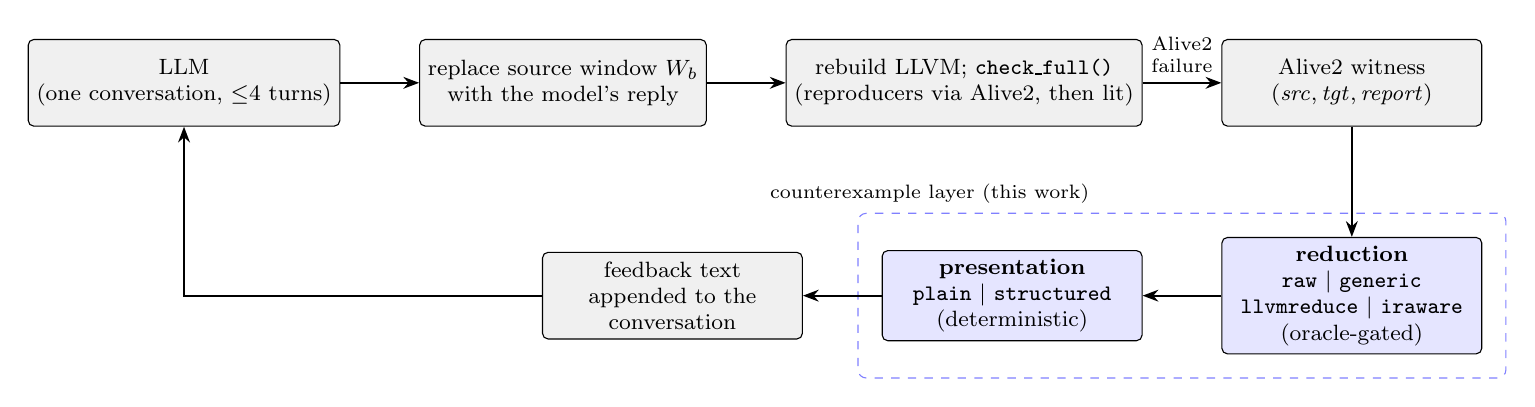
\begin{tikzpicture}[
  font=\footnotesize,
  box/.style={draw, rounded corners=2pt, align=center, minimum height=11mm, minimum width=33mm, inner sep=3pt},
  inh/.style={box, fill=black!6},
  ours/.style={box, fill=blue!10},
  arr/.style={-{Stealth[length=2mm]}, thick},
  lbl/.style={font=\scriptsize, align=center}]
\node[inh] (llm) {LLM\\(one conversation, $\le$4 turns)};
\node[inh, right=10mm of llm] (patch) {replace source window $W_b$\\with the model's reply};
\node[inh, right=10mm of patch] (check) {rebuild LLVM; \texttt{check\_full()}\\(reproducers via Alive2, then lit)};
\node[inh, right=10mm of check] (wit) {Alive2 witness\\$(\mathit{src},\mathit{tgt},\mathit{report})$};
\node[ours, below=14mm of wit] (red) {\textbf{reduction}\\\cn{raw} $\mid$ \cn{generic}\\\cn{llvmreduce} $\mid$ \cn{iraware}\\(oracle-gated)};
\node[ours, left=10mm of red] (pres) {\textbf{presentation}\\\cn{plain} $\mid$ \cn{structured}\\(deterministic)};
\node[inh, left=10mm of pres] (fb) {feedback text\\appended to the\\conversation};
\draw[arr] (llm) -- (patch);
\draw[arr] (patch) -- (check);
\draw[arr] (check) -- node[above, lbl]{Alive2\\failure} (wit);
\draw[arr] (wit) -- (red);
\draw[arr] (red) -- (pres);
\draw[arr] (pres) -- (fb);
\draw[arr] (fb.west) -| (llm.south);
\begin{scope}[on background layer]
\node[draw=blue!50, dashed, rounded corners=3pt, fit=(red)(pres), inner sep=3mm, label={[font=\scriptsize]above left:counterexample layer (this work)}] {};
\end{scope}
\end{tikzpicture}
\caption{The counterexample layer (blue) inside the inherited repair loop (grey). Reduction and presentation are independent factors. A passing check ends the run. Failures other than Alive2 refinement failures (build, lit, unmatched window) bypass the layer, and their log text is passed through unchanged. The \cn{baseline} condition replaces both blue boxes with a fixed sentence.}
\label{fig:arch}
\end{figure*}

\subsection{The preserved property: the oracle}

Every reducer proposes a candidate pair and asks an oracle whether the violation survives. The oracle runs \texttt{alive-tv} on the candidate and compares the result with the violation reported for the original pair. That violation is described by the function name, the Alive2 error class (for example, ``Target is more poisonous than source''), and a coarse \emph{kind} of target-side outcome (poison, undef, UB, or a concrete wrong value) inferred from the report. Three strictness levels are defined:
\begin{itemize}
\item \cn{any\_failure}: some refinement failure is still reported, in any function;
\item \cn{error\_class} (the default): a failure with the same error class is reported in the same function;
\item \cn{error\_class\_and\_kind}: additionally, the target-side outcome kind matches.
\end{itemize}

A candidate that Alive2 cannot parse or type-check is rejected, as is a candidate whose run errors without reporting a violation. Matching an error class is weaker than preserving the original root cause or the original execution, because two different inputs or two different flags can trigger the same class in the same function. At \cn{any\_failure}, the reducer may drift onto an unrelated bug. A reduced witness is therefore a valid counterexample with the same error class in the same function. It is not a proof of equivalence with the original witness, and it is not guaranteed to be globally minimal.

\subsection{Baseline reducers}

\textbf{\cn{generic}.} The reduction units are the lines of both files. A variant of \texttt{ddmin} proposes subsets and complements, and each candidate is rendered by concatenating the surviving lines of each file. The reducer has no notion that the files are versions of one function, so candidates that contain lines from only one side are simply rejected. Relative to the original algorithm~\cite{zeller2002dd}, the implementation jumps directly to single-element granularity when no subset or complement succeeds, instead of doubling the number of chunks.

\textbf{\cn{llvmreduce}.} \texttt{llvm-reduce} accepts one file and one interestingness test, so the pairing is supplied from outside. The wrapper first reduces the source with the target held fixed. It then reduces the target with the \emph{already reduced} source held fixed, and finally it checks the reduced pair together. The tool's own passes are unmodified. Each candidate spawns a separate process that runs the oracle and returns only an exit status, so the tool never sees the violation or the other file. This isolates ``understands IR'' from ``understands the counterexample.''

\subsection{The IR-aware reducer}

The reducer operates on a parsed model of the module (Section~\ref{sec:impl}) rather than on text. It differs from the baselines in three ways.

\emph{Tandem editing.} Source and target are two versions of one function. Edits are applied to both and matched by SSA name, so that deleting a value on one side deletes the same-named value on the other.

\emph{Dependency-closed candidates.} Instead of deleting lines, the reducer chooses a set of values to \emph{keep}. It then closes this set over def-use edges, the operands of terminators and returns, and the branch conditions of every block from which the kept values are reachable. Everything outside the closure is removed. This avoids dangling uses by construction. It does not guarantee a valid module, because type or phi-edge inconsistencies and parser misreads remain possible, which is why every candidate still goes to the oracle.

\emph{Counterexample-derived seeds.} The verifier report provides three kinds of information. First, it supplies the \emph{seeds}, which are the values the reducer must keep: values whose trace values differ between source and target, values that are poison, undef, or UB on the target side, and values that appear only on the source side. The values returned by the source function are added to this set. Second, it records the \emph{executed blocks} on the source side, which determine the branch to fold. Third, it gives the \emph{type} of each value printed in the example and traces, which is used when a value is promoted to a parameter.

\begin{table}[t]
\caption{Passes of the IR-aware reducer, in application order. Every proposal is gated by the oracle.}
\label{tab:passes}
\centering\footnotesize
\begin{tabular}{@{}p{2.75cm}p{4.75cm}@{}}
\toprule
Pass & Proposal \\
\midrule
\cn{dce} & delete values that no instruction reads, except seeds (up to 16 sweeps) \\
\cn{fold-branches} & replace a conditional branch by an unconditional one to the successor that the source trace entered, when exactly one successor was entered \\
\cn{prune-blocks} & delete blocks unreachable from entry, pruning \texttt{phi} edges \\
\cn{simplify-cfg} & replace single-edge \texttt{phi}s by their value; splice a block into its sole unconditional predecessor (up to 32 steps) \\
\cn{slice} & pin the seeds; \texttt{ddmin} over the remaining source values, each subset closed as above and applied to both sides \\
\cn{promote-operands} & replace a non-seed, non-\texttt{phi} value defined on both sides by a fresh parameter of the trace's type, then delete dead producers \\
\cn{drop-params} & remove parameters unused on both sides \\
\cn{strip-flags} & \texttt{ddmin} over the \texttt{nsw}, \texttt{nuw}, \texttt{exact}, \texttt{inbounds}, \texttt{nneg}, \texttt{disjoint}, \texttt{samesign} and fast-math flags on either side \\
\bottomrule
\end{tabular}
\end{table}

Table~\ref{tab:passes} lists the passes, and Algorithm~\ref{alg:iraware} gives the driver. Branch folding is unsound in general (for instance, when the condition is poison), which is one reason the oracle gates it.

\textbf{Operand promotion generalizes the witness.} A fresh parameter may take any value of its type, so the reduced pair may describe an execution that the original program cannot reach. The oracle guarantees that the violation is preserved, but not that it remains relevant to the original bug. Promotion is therefore separately switchable (\texttt{--no-promotion}) and is the subject of the ablation in RQ6.

\begin{algorithm}[t]
\caption{IR-aware reduction (as implemented)}
\label{alg:iraware}
\begin{algorithmic}[1]
\Require $\mathit{src},\mathit{tgt}$, parsed violation $R$ (function $f$), oracle $\mathcal O$ with budget $B$, flag \textsc{promote}, $\mathit{max\_rounds}{=}4$
\State parse both modules; \textbf{if} parsing fails or $f$ is missing in either \textbf{return} unreduced with an error
\State $\mathit{seeds}\gets$ diverging, target-poison/undef/UB, and source-only trace values $\cup$ values returned by $f_{src}$
\State $\mathit{types}\gets$ value types in $R$;\; $\mathit{exec}\gets$ source-side blocks entered in $R$
\State $S\gets(f_{src},f_{tgt})$;\; $\mathit{applied}\gets\emptyset$
\For{$\mathit{round}=1$ \textbf{to} $\mathit{max\_rounds}$}
  \State $\mathit{progress}\gets\textbf{false}$
  \For{\textbf{each} pass $P$ \textbf{in} \cn{dce}, \cn{fold-branches}, \dots, \cn{strip-flags}}
    \If{$\mathcal O$.exhausted} \textbf{break} \EndIf
    \State $S'\gets P(S)$ \Comment{each accepted proposal: $\mathcal O(\textsc{render}(S'))$ preserves the violation}
    \If{$S'\neq\bot$} $S\gets S'$;\; $\mathit{applied}\gets\mathit{applied}\cup\{P\}$;\; $\mathit{progress}\gets\textbf{true}$ \EndIf
  \EndFor
  \If{\textbf{not} $\mathit{progress}$ \textbf{or} $\mathcal O$.exhausted} \textbf{break} \EndIf
\EndFor
\If{$\mathit{applied}\neq\emptyset$ \textbf{and not} $\mathcal O(\textsc{render}(S))$} \textbf{return} the original pair \EndIf
\State \Return $\textsc{render}(S)$
\end{algorithmic}
\end{algorithm}

\subsection{Presentation}

\textbf{Plain.} The text consists of ``Source:'' followed by the IR of the (possibly reduced) source, ``Target:'' followed by the target IR, and then Alive2's own report from the line ``Transformation doesn't verify!'' onward. The report includes the example input, the per-value traces for both sides, and the final values. When the pair was reduced, the report comes from re-running Alive2 on the reduced pair, so the trace describes the IR that is shown.

\textbf{Structured.} The same IR pair is shown, followed by labelled sections: bug type, verification result, violated property, a diff of source and target keyed by SSA name rather than by line, critical values (the seeds), the dependency chain of the seeds in the source, the blocks entered, the counterexample input, the first divergences between source and target values, memory state when present, and an interpretation. The interpretation is a fixed template per Alive2 error class, filled with values from the report. Six error classes have templates, and other classes receive a one-sentence fallback. A further sentence names any flag that is present in the target and absent in the source. No text is produced by a model. Structured presentation is not information-neutral. It omits the per-value traces that the plain report contains, and it adds derived sections (the diff, the dependency chain, and the interpretation). Differences between \cn{plain} and \cn{structured} are therefore differences in both organization and content.

\subsection{Fallbacks and stopping}

Reduction returns the unreduced pair in any of four cases: (i) a module cannot be parsed or the function is absent from either module; (ii) the oracle budget is exhausted (the default is 400 \texttt{alive-tv} calls per reduction, including the final check); (iii) the final check of a reduced pair fails; or (iv) the reduced pair fails a separate re-verification before rendering.

The IR-aware reducer stops after at most four rounds of the eight passes, when a round makes no progress, or when the budget is exhausted. It does not claim to reach a fixed point. Within a pass, \texttt{ddmin} ends at a subset that is 1-minimal with respect to that pass's units, unless the budget stops it first. Because the final check is itself an oracle call, a reduction that exhausts the budget is discarded in full. In a code-path check with a verifier stubbed to accept every candidate, budgets of 1 to 3 calls returned the original 28-instruction pair, whereas budgets of 400 and unlimited returned a 4-instruction pair; this check exercises the code path and is not a measurement of any reduction. The \texttt{llvm-reduce} wrapper is additionally capped at 600~s of wall-clock time per side.

%=====================================================================
\section{Implementation}
\label{sec:impl}
%=====================================================================

The implementation is the \texttt{ce} Python package in the project repository\footnote{\url{https://github.com/Tanish-Desai/better-compiler}, branch \texttt{feat/counterexample-toolkit}, commit \texttt{b1d6bfe6236a0da7d7aeb85ae2a03bd2518dadbd}, which was the branch tip on 2026-10-06.}~\cite{betterCompiler2026}. The benchmark is a vendored copy of \emph{llvm-apr-benchmark} whose upstream commit is not recorded. Alive2 is built from a pinned commit (\texttt{f9a4f02f}) against LLVM~21 development packages in an Ubuntu~22.04 image.

\textbf{Alive2 interface and parser.} \texttt{alive-tv} is invoked with \texttt{--disable-undef-input}, as in the benchmark, after \texttt{noalias} and \texttt{nofree} are removed from both files (the benchmark's own pre-pass). The parser splits the output at the separator line and reads the error class from the \texttt{ERROR:} line. It also reads the example, the two traces (including the \texttt{Jump to} annotations), the source and target values, and the memory-state blocks. Alive2's output format is not a documented interface. Anything unrecognized stays in the raw text, and output with no parseable section is reported as a tool error.

\textbf{IR model.} The model is line-oriented and is not an LLVM parser. It separates the module preamble from function definitions and splits each function into parameters, blocks, and instructions, recording result names, opcodes, value operands, and label operands. Bracketed instructions that span several lines are joined. Anything that the model does not represent must survive parse-then-print unchanged, and the repository's check (\texttt{scripts/check\_ir\_roundtrip.py}) confirms this for all 1{,}462 reproducer bodies in the 491 vendored issue files, which round-trip byte for byte. This verifies the identity property only. It does not establish that edits are correct. Edit correctness is delegated to the oracle: an IR-model error typically surfaces as a rejected candidate and hence a weaker reduction, although undetected drift remains possible because the oracle preserves an error class rather than the original witness (Section~\ref{sec:method}). Source and target are paired by SSA name, which assumes that the target printed by \texttt{opt} keeps the names used in the source.

\textbf{Feedback assembly.} The runner passes each failed check to \texttt{normalize\_feedback}, which selects the first failing test. If that test's log is an Alive2 result, the condition's text is built from it. Otherwise the log string is passed through, subject to a $10^9$-character cap that is effectively nonbinding in this setting. In this snapshot, the reduction oracle and the re-verification call \texttt{alive-tv} without the per-test \texttt{additional\_args} that the benchmark supplies (for example, \texttt{-src-unroll=4 -tgt-unroll=4}). Five of the 24 sampled bugs carry such arguments (126012, 114879, 91369, 180870, and 91957), and the effect of this omission on their reductions has not been measured.

\textbf{Repair loop.} The runner is adapted from the benchmark's example loop rather than invoking that implementation unchanged. It follows the hint-based path rather than the bisection path. The system prompt is ``You are an LLVM maintainer'' plus a format requirement. The first user turn states the bug type and component, the issue title (without the body), the feedback text, and a source window with a prefix and suffix requirement. The window is the line range of the first hinted file, extended by 30 lines on each side and read from the base commit. For the 24 sampled bugs it spans 66 to 149 lines before clipping at file boundaries.

The reply replaces the window by string substitution, and the model is told if the window is not found. Before each turn the tree is reset to the base commit, so a reply is a patch relative to the original window rather than to the previous reply. Subsequent turns append the feedback and the format requirement to the same conversation. A reply identical to the window receives no special handling: it is applied, built, and checked like any other reply. Differences from the benchmark's loop in this snapshot include omitting the function name from the prompt, returning a fixed message on a window mismatch, skipping bugs that do not reproduce, writing no record when the provider fails before the first reply, and rendering the \cn{raw-plain} text differently from the benchmark's JSON dump of the failed test.

\textbf{Model client.} The client is OpenAI-compatible, with a 300~s timeout. No maximum-token limit is supplied, and no \texttt{top\_p} parameter is passed. The temperature is read from \texttt{LAB\_LLM\_TEMP} (default 0.8). The model is selected through environment variables: the repository's code defaults to \texttt{deepseek-reasoner}, whereas its documentation names open-weight models. The model identifier and revision, quantization, serving stack, maximum context, \texttt{top\_p}, and output limit are therefore not fixed by this snapshot and will be reported with the results.

\textbf{Tests.} The repository contains 63 tests. In an environment without \texttt{alive-tv} and \texttt{llvm-reduce}, 45 run and pass, and the 18 integration tests that exercise the reducers against the real verifier are skipped. The repository documentation reports all 63 passing in the project container.

%=====================================================================
\section{Experimental Design and Evaluation Protocol}
\label{sec:design}
%=====================================================================

The protocol below is the one documented and coded in the repository; it has not yet been run. A document committed on 2026-09-04, before any run record existed in the repository, fixes the repeat count, the test, and the primary family of comparisons. This is a preregistration only in the sense of repository history; it was not deposited in an external registry.

\subsection{Population}

\begin{table}[t]
\caption{From the full benchmark to the sample, counted from the vendored dataset files.}
\label{tab:funnel}
\centering\footnotesize
\begin{tabular}{@{}p{6.4cm}r@{}}
\toprule
Stage & Bugs \\
\midrule
Dataset files (crash 340, miscompilation 142, hang 9) & 491 \\
Miscompilations checked with Alive2 (7 are \texttt{lli}-only) & 135 \\
\ldots\ with \texttt{is\_single\_func\_fix} (eligible subset) & 100 \\
\ldots\ minus bootstrap bug 115575 (sampling pool) & 99 \\
Sample: 8 per tier, tiers of 33 & 24 \\
Analyzed (recorded under all conditions) &  \\
\bottomrule
\end{tabular}
\end{table}

A bug is eligible if it is a miscompilation, every reproducer is checked by Alive2 rather than \texttt{lli}, and the reference fix touches one function. The counterexample conditions require the first filter, and the runner skips multi-function fixes. The pool excludes bug 115575, which was used during harness development. The pool is sorted by hint-region size (the number of lines covered by the bug-location hints), then by reproducer size, then by identifier, and it is cut into three tiers of 33 bugs. Within each tier, bugs are drawn round-robin across the first hinted component, so that InstCombine (45 of the 100 eligible bugs) does not dominate. The procedure is deterministic, and re-running the selection script reproduces the committed list. The tier labels in the repository (easy, medium, hard) describe the size of the hint region and reproducer, not measured difficulty for any model.

The sample has 16 distinct primary component labels, one of which is a placeholder for a bug with no component hint. Eleven of the 24 bugs have knowledge cutoffs in 2025 or 2026. Results will be reported over this subset of miscompilations only, not over the whole benchmark. The runner additionally skips a bug whose failure does not reproduce at its base commit, so the analyzed count may be below 24.

\subsection{Conditions}

\begin{table}[t]
\caption{The nine conditions. The \cn{baseline} condition receives a fixed sentence and no counterexample.}
\label{tab:conditions}
\centering\footnotesize
\begin{tabular}{@{}lll@{}}
\toprule
Reduction & \cn{plain} & \cn{structured} \\
\midrule
(none) & \cn{baseline} & --- \\
\cn{raw} & \cn{raw-plain} & \cn{raw-structured} \\
\cn{generic} & \cn{generic-plain} & \cn{generic-structured} \\
\cn{llvmreduce} & \cn{llvmreduce-plain} & \cn{llvmreduce-structured} \\
\cn{iraware} & \cn{iraware-plain} & \cn{iraware-structured} \\
\bottomrule
\end{tabular}
\end{table}

\textbf{Held constant.} Across conditions, the model, the system and user prompt text apart from the feedback, the source window, the maximum number of iterations (4), the oracle budget (400 calls), the oracle strictness (\cn{error\_class}), and the temperature are identical. The iteration limit, oracle budget, strictness, and temperature are recorded in every run record. The deliberate exceptions are the feedback text itself and, as a consequence, the prompt length. Non-Alive2 failures are identical across conditions, so the treatments differ only on turns where the failing check is an Alive2 refinement failure. LLM sampling is not seeded.

\subsection{Procedure and budget}

Each of the 24 bugs is run under each of the 9 conditions for 3 trials (648 runs). An ablation of the two \cn{iraware} conditions with promotion disabled adds 144 runs, for 792 in total. A run lasts at most four turns, and each turn consists of a rebuild and a lit run. The runner iterates bug-major so that one build per base commit can be reused, and it skips cells whose record already exists. A cell of a bug and condition that has no record (for example, because the provider failed before the first reply) is left empty rather than recorded as a failure.

\subsection{Success criterion}
\label{sec:success}

A run succeeds on the first turn at which the benchmark's \texttt{check\_full()} returns true. That function performs three steps. (i) It builds LLVM with CMake and Ninja in \texttt{RelWithDebInfo} mode with assertions enabled, for the X86, RISCV, AArch64, SystemZ, Hexagon, PowerPC, and NVPTX targets. (ii) It runs every reproducer test through \texttt{opt} and requires Alive2 to report zero incorrect transformations, zero failed-to-prove transformations, and zero errors. (iii) It checks out the \texttt{llvm/test} tree of the fix commit and runs \texttt{llvm-lit} over the directories listed for that bug (one directory for 23 of the 24 sampled bugs and four for bug 114879), stopping at the first failure, with a 300~s limit.

This is a plausibility criterion, bounded by Alive2's unroll limit and by the listed test directories. It is not a proof of correctness, and it does not cover the whole LLVM regression suite. Because the \emph{llvm-harness} expert review found a substantial share of benchmark-passing patches to be invalid~\cite{zheng2026harness}, we call a passing patch \emph{plausible}. The repository does not plan a manual review of patches.

\subsection{Metrics}

The primary outcome is the bug-level success indicator \emph{pass@3}: a bug counts as repaired under a condition if at least one of its three trials succeeds. Here pass@3 denotes this observed per-bug indicator. When all three trials of a cell exist, it coincides with the unbiased pass@$k$ estimator for $n=k=3$~\cite{yang2026reducefix}, but it is not an estimate from a larger sample. \emph{Pass@1}, the fraction of individual runs that succeed, is reported alongside it. The bug is the unit of analysis: repeated trials reduce per-cell noise but do not add independent bugs. The secondary measures are as follows.
\begin{itemize}
\item Iterations to repair (LLM turns until success) and the build and verifier-call counts that scale with it. Runs that do not succeed are censored at the iteration limit, so the repository's unconditional mean is not by itself an efficiency estimate. The analysis of this measure is not specified in the repository.
\item Reducer measures: instructions, lines, blocks, values, and characters before and after reduction, oracle calls, accepted and rejected candidates, tool failures, and seconds.
\item LLM prompt and completion tokens as reported by the server, and an \emph{estimated} feedback size (characters divided by four), which is used only to compare conditions.
\item Wall-clock time, which is descriptive only.
\end{itemize}

\subsection{Inference}

Four comparisons are primary, each in a direction stated beforehand: \cn{iraware-plain} versus \cn{generic-plain}, \cn{iraware-plain} versus \cn{llvmreduce-plain}, \cn{iraware-structured} versus \cn{iraware-plain}, and \cn{raw-plain} versus \cn{baseline}. For a pair, let $b$ be the number of bugs repaired only under the hypothesized-better condition and $c$ the number repaired only under the other. The exact one-sided McNemar test conditions on $n=b+c$ and uses the binomial tail
\begin{equation}
p=\sum_{i=b}^{n}\binom{n}{i}2^{-n}.
\end{equation}
The four $p$-values are adjusted together with the Benjamini--Hochberg procedure~\cite{benjamini1995fdr} at $\alpha=0.05$. For every comparison, the analysis script also prints the repaired counts, $b$, $c$, the paired difference in proportions, an odds ratio, and a two-sided $p$-value. We report $b$, $c$, and the difference regardless of the $p$-value, and we do not read a non-significant result as evidence of no effect. The other 32 pairs are exploratory and are reported uncorrected and descriptively. The ablation compares each \cn{iraware} condition with itself under promotion on and off, as a separate family of two tests. The script tests the one-sided hypothesis that promotion on is better, so a benefit of disabling promotion would not be detected by that test.

Fewer than five discordant bugs cannot yield $p<0.05$ one-sided at any split, and $n=24$ limits power. Under assumed per-attempt rates of 0.12--0.35 and a per-bug difficulty multiplier, the repository's simulation gives power between roughly 0.10 and 0.57 at three trials. The assumptions are the authors' and are based on reported frontier-agent rates rather than on data from this setup. The comparison is therefore best read as a pilot-scale screen. Conditions should have equal numbers of trials before pass@3 is compared.

%=====================================================================
\section{Results}
%=====================================================================

The experimental sweep has not been run, so every cell below is intentionally left blank. No value, ranking, or significance marker is implied.

\begin{table}[t]
\caption{Repair outcomes by condition.}
\label{tab:main}
\centering\footnotesize
\begin{tabular}{@{}lcccc@{}}
\toprule
Condition & Bugs & Pass@3 & Pass@1 & Iters.\ \\
\midrule
\cn{baseline} &  &  &  &  \\
\cn{raw-plain} &  &  &  &  \\
\cn{raw-structured} &  &  &  &  \\
\cn{generic-plain} &  &  &  &  \\
\cn{generic-structured} &  &  &  &  \\
\cn{llvmreduce-plain} &  &  &  &  \\
\cn{llvmreduce-structured} &  &  &  &  \\
\cn{iraware-plain} &  &  &  &  \\
\cn{iraware-structured} &  &  &  &  \\
\bottomrule
\end{tabular}
\end{table}

\begin{table}[t]
\caption{Prespecified comparisons (hypothesized-better condition first).}
\label{tab:tests}
\centering\footnotesize
\setlength{\tabcolsep}{3pt}
\begin{tabular}{@{}p{3.2cm}ccccc@{}}
\toprule
Comparison & $b$ & $c$ & Diff. & $p$ & $p_{\mathrm{BH}}$ \\
\midrule
\cn{iraware-plain} vs \\ \cn{generic-plain} &  &  &  &  &  \\
\cn{iraware-plain} vs \\ \cn{llvmreduce-plain} &  &  &  &  &  \\
\cn{iraware-structured} vs \\ \cn{iraware-plain} &  &  &  &  &  \\
\cn{raw-plain} vs \\ \cn{baseline} &  &  &  &  &  \\
\bottomrule
\end{tabular}
\end{table}

\begin{table}[t]
\caption{Reducer behavior on the first witness of each bug.}
\label{tab:reducers}
\centering\footnotesize
\begin{tabular}{@{}lcccc@{}}
\toprule
Reduction & Ratio (instr.) & Oracle calls & Seconds & No reduction \\
\midrule
\cn{generic} &  &  &  &  \\
\cn{llvmreduce} &  &  &  &  \\
\cn{iraware} &  &  &  &  \\
\bottomrule
\end{tabular}
\end{table}

\begin{table}[t]
\caption{Operand-promotion ablation.}
\label{tab:ablation}
\centering\footnotesize
\begin{tabular}{@{}lccc@{}}
\toprule
Condition & Pass@3 (on/off) & $b/c$ & Ratio (on/off) \\
\midrule
\cn{iraware-plain} &  &  &  \\
\cn{iraware-structured} &  &  &  \\
\bottomrule
\end{tabular}
\end{table}

%=====================================================================
\section{Discussion}
%=====================================================================

Interpretation has to wait for results. The questions that the interpretation must address are listed here so that they are not decided after the fact.
\begin{itemize}
\item Whether the difference, if any, between \cn{iraware-plain} and \cn{generic-plain} tracks prompt length, which can be examined by comparing the length distributions of the two conditions.
\item Whether \cn{llvmreduce-plain} behaves like \cn{iraware-plain} on bugs where both reduce substantially.
\item Whether any difference between \cn{plain} and \cn{structured} is attributable to organization or to the content that differs (Section~\ref{sec:method}).
\item Whether the \cn{iraware} outcomes depend on operand promotion, and whether reduced witnesses that used promotion describe executions of the original reproducer.
\item Whether bugs on which reduction fell back to the unreduced pair differ in outcome from the rest.
\item Which bugs are repaired under \cn{baseline}, since a model that repairs a bug from the title and the window alone leaves no room for feedback to matter.
\end{itemize}

%=====================================================================
\section{Threats to Validity and Limitations}
\label{sec:threats}
%=====================================================================

The following are properties of the implementation or the design that can be established without results. Their effect on outcomes has not been measured.

\textbf{Witness generalization.} Operand promotion can yield witnesses that describe unreachable executions. Only the ablation addresses this, and only through repair outcomes rather than through judgments of relevance.

\textbf{What the oracle preserves.} Equal error class in the same function does not imply equal root cause. The default strictness level was chosen as a compromise, results at other levels are not comparable, and only one level is planned.

\textbf{Bounded verification.} A reduced witness is a counterexample under the same bounded semantics, and the oracle cannot detect violations that require more loop iterations than Alive2's unroll bound. The omitted \texttt{additional\_args} on five sampled bugs (Section~\ref{sec:impl}) is a specific instance of this limitation in the present snapshot.

\textbf{Parser and model coverage.} The IR model is line-oriented, and the round-trip check does not test edits. When a parser error produces invalid IR or destroys the preserved violation, the oracle rejects the candidate, which typically turns the error into a missed reduction. However, because the oracle preserves an error class rather than semantic equivalence to the original witness, undetected semantic drift remains possible. Missed reductions make \cn{iraware} resemble \cn{raw} on the affected bugs. Unreduced fallbacks will be counted in the results.

\textbf{Reduction failures and budget.} A reduction that exhausts the budget is discarded rather than returned, so a tight budget biases the outcome toward unreduced witnesses. The budget of 400 calls is shared by the reducers in different ways: the \texttt{llvm-reduce} wrapper counts its subprocess calls against the same budget and additionally has a wall-clock cap that the other reducers lack.

\textbf{Source and target name matching.} Tandem editing and the structured diff assume that names correspond between the reproducer and the IR printed by the patched \texttt{opt}. Renumbered unnamed values or renamed instructions would appear as unrelated additions and removals. Only the target function with the reported name is reduced, and other functions in the module are left untouched.

\textbf{Prompt length and content.} Conditions differ in prompt length by construction. The \cn{generic} condition controls for length only if it actually shortens the prompt. The repository documents a single hand-built case in which it removed nothing, and whether it shortens real witnesses is unmeasured. In addition, \cn{structured} changes content as well as layout. Length is estimated as characters divided by four.

\textbf{Treatment reach.} Only Alive2 failures are treated. Build and lit failures are passed through verbatim and untruncated, so their length varies independently of the condition.

\textbf{Model dependence and sampling.} One model and one temperature (0.8 by default) are planned, and the client passes no \texttt{top\_p} parameter. The effect of feedback form may depend on model scale and training, and repeated sampling adds noise that three trials only partly average out. The model configuration is not yet fixed.

\textbf{Benchmark contamination.} The sampled bugs date from 2024-02 to 2026-02, so a model trained afterward may have seen the fixes. The harness records a self-declared model cutoff date that it does not verify, and we therefore make no claim about contamination-free evaluation. Contamination affects all conditions for a given bug, but it could produce a ceiling at which no condition is discordant.

\textbf{Localization hints.} The window is built from the benchmark's bug-location hints, which the benchmark describes as best-effort and which appear to be derived from the reference fix. The prompt also includes the issue title, which for some sampled bugs names the faulty flag or pass. The experiment therefore measures repair given a localized window, not autonomous localization. The window does not respect statement boundaries, so a model may receive a truncated function.

\textbf{Validation scope.} The \texttt{check\_full()} function bounds success as described in Section~\ref{sec:success}, and the Alive2 check passes only on the reproducers that the benchmark lists. A patch can be plausible and still incorrect, as the \emph{llvm-harness} review found in its own setting~\cite{zheng2026harness}.

\textbf{Departures from the inherited loop.} The runner differs from the benchmark's example loop (Section~\ref{sec:impl}). In particular, the \cn{raw-plain} condition does not reproduce the benchmark's prompt exactly, and the resulting rates are not comparable to published rates for the benchmark.

\textbf{Naming effects.} The reducer introduces parameter names of the form \texttt{\%ce.argN}. We know of no evidence on the effect of such names on models for IR. Evidence from Java repair shows sensitivity to renaming for fine-tuned models~\cite{rabbi2026hej}, but it need not transfer to this setting.

\textbf{Statistical resolution.} With 24 bugs, a non-significant comparison is uninformative about the absence of an effect. Pass@3 and pass@1 can disagree, and iterations to repair are conditional on repair. The contrast of the full method (\cn{iraware-structured}) against \cn{baseline} is not in the primary family and is exploratory.

\textbf{Scope.} Any results will concern single-function miscompilations checked by Alive2. They will not extend to crashes, hangs, multi-function fixes, or miscompilations checked by execution.

%=====================================================================
\section{Conclusion}
%=====================================================================

We specified a layer that reduces and structures Alive2 counterexamples inside an existing LLVM repair loop. The layer has two independent factors, three reduction strategies of increasing counterexample awareness, a deterministic renderer, and an oracle that bounds what a reduction may change. We also specified a nine-condition protocol with a paired, prespecified analysis. The implementation's IR model round-trips the benchmark's reproducers byte for byte, but the behavior of the reducers on real witnesses has not yet been measured, the model is not fixed, and no repair outcome exists. Whether any condition repairs more bugs than another is therefore unknown. The next steps are to resolve the verifier-argument plumbing and the model configuration, to run the nine-condition pilot on the excluded bootstrap bug to check that the loop, the prompts, and the fallbacks behave as described, and then to run the sweep and fill Tables~\ref{tab:main}--\ref{tab:ablation}.

\bibliographystyle{IEEEtran}
\bibliography{references}

\end{document}
